\documentclass[11pt]{article}
\usepackage[T1]{fontenc}
\usepackage{lmodern,amsmath,amssymb,mathtools,mathrsfs,booktabs,longtable,array,microtype,graphicx}
\usepackage[a4paper,margin=24mm]{geometry}
\usepackage[hidelinks,hypertexnames=false]{hyperref}
\usepackage{xurl}
\setlength{\emergencystretch}{3em}
\providecommand{\tightlist}{\setlength{\itemsep}{0pt}\setlength{\parskip}{0pt}}
\title{Arithmetic frame nonsingularity, native determinant returns, and signed-cover descent}
\author{The Clankers}
\date{20 September 2026}

\begin{document}
\maketitle
\begin{abstract}
For positive integral Erd\H{o}s--Straus witnesses, this reader proves a
three-character sufficient condition for nonsingularity of the original odd
receiving frame.  The condition comprises exactly 3,456 reduced residue
classes modulo 521,220, and an independent reconstruction checks all 163
sorted witnesses at five diagnostic primes.  An exact arithmetic-descent
example at the genuine witness $(13;4,18,468)$ has no original signed lift
over $\mathbb F_{61}$, eight lifts over $\mathbb F_{61^2}$, and eight rational
points on its nonsquare twist.  Adjacent tracks derive a sharp paired native
determinant return and finite heat-action remainder certificates while keeping
the two heat functions and every metric distinct.  No universal occupancy,
RH, or global endpoint conclusion is inferred.
\end{abstract}

\section*{Verification boundary}
The independent local checker replays Tracks I and IV with 923 exact checks.
The supplied packet reports executable checks for Tracks II and III, but those
scripts were not among the received files; their proofs are retained below
without relabelling the received receipt as a local run.

\begin{figure}[p]
\centering
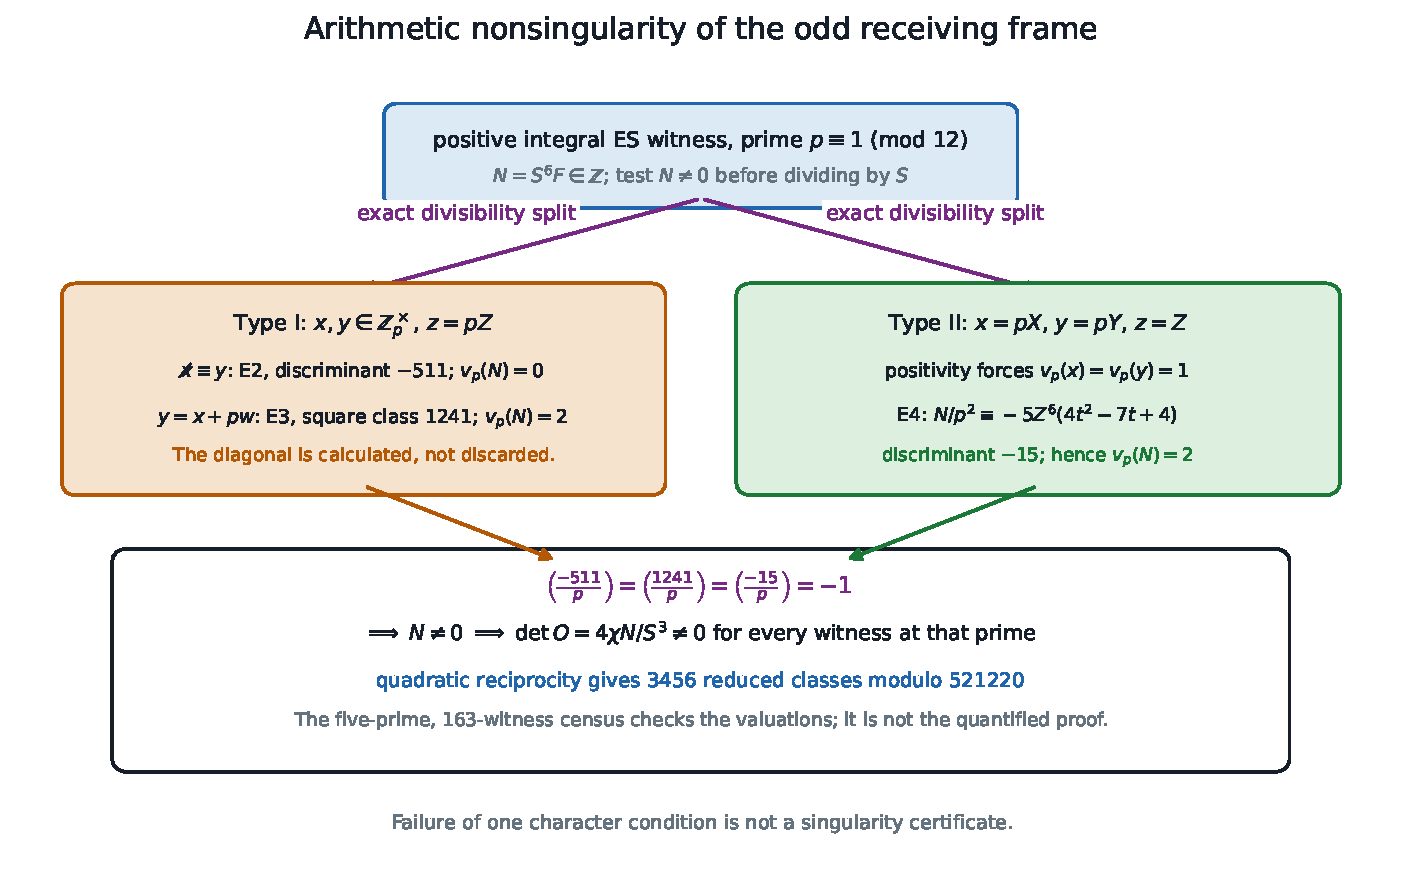
\includegraphics[width=\textwidth]{figures/arithmetic-frame-sieve.pdf}
\caption{The exhaustive denominator-valuation split and the three quadratic
obstructions used in Theorem E.  A failed character condition is not a
singularity certificate.}
\end{figure}
\clearpage

\begin{figure}[p]
\centering
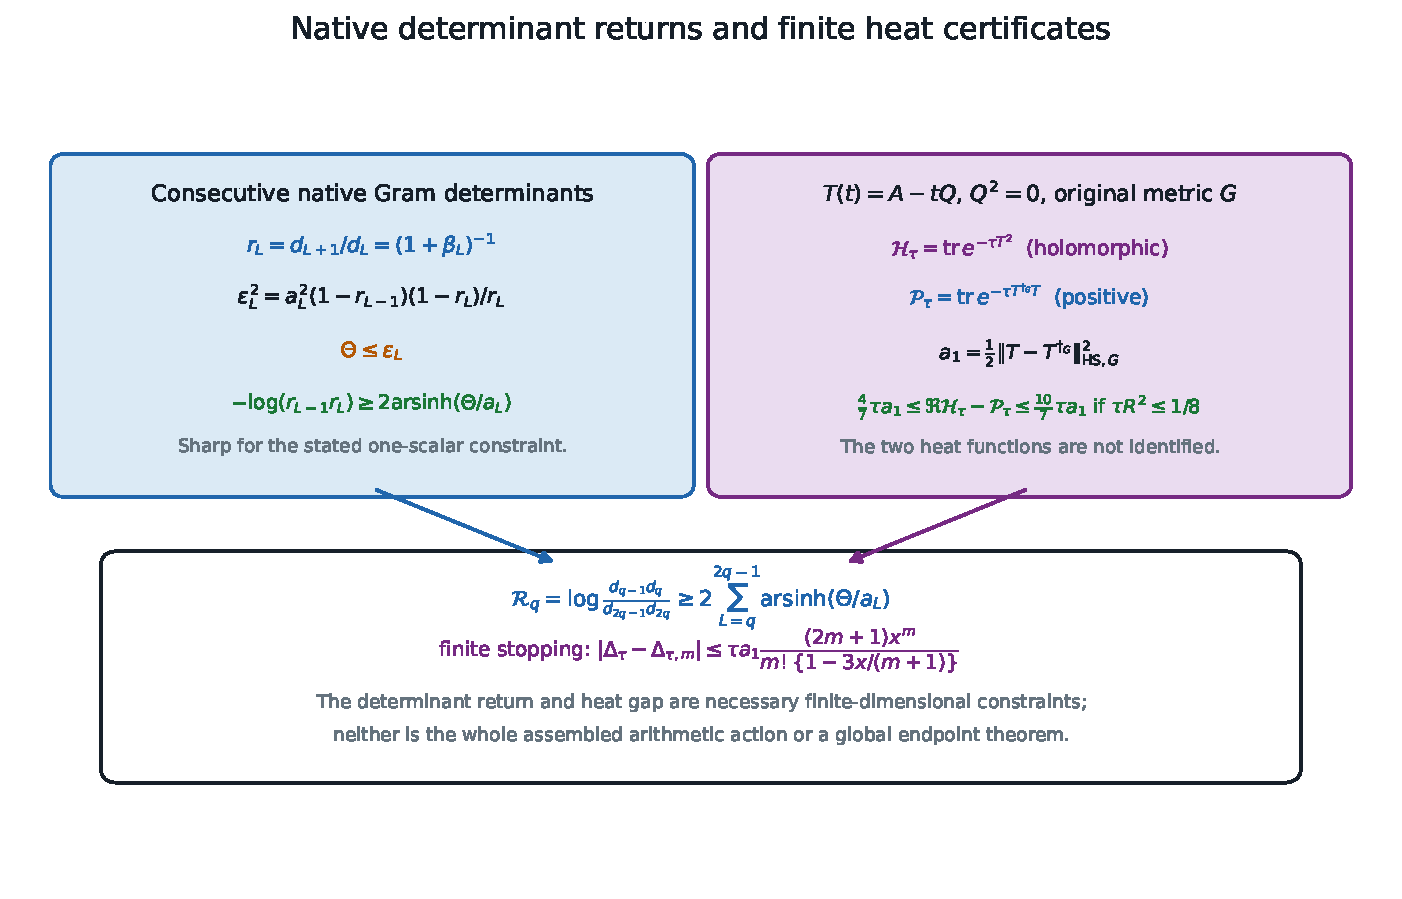
\includegraphics[width=\textwidth]{figures/determinant-heat-mechanism.pdf}
\caption{The exact consecutive-determinant identity, its sharp two-ratio
consequence, and the separate finite heat actions with their proved
small-time boundary.}
\end{figure}
\clearpage

\begin{figure}[p]
\centering
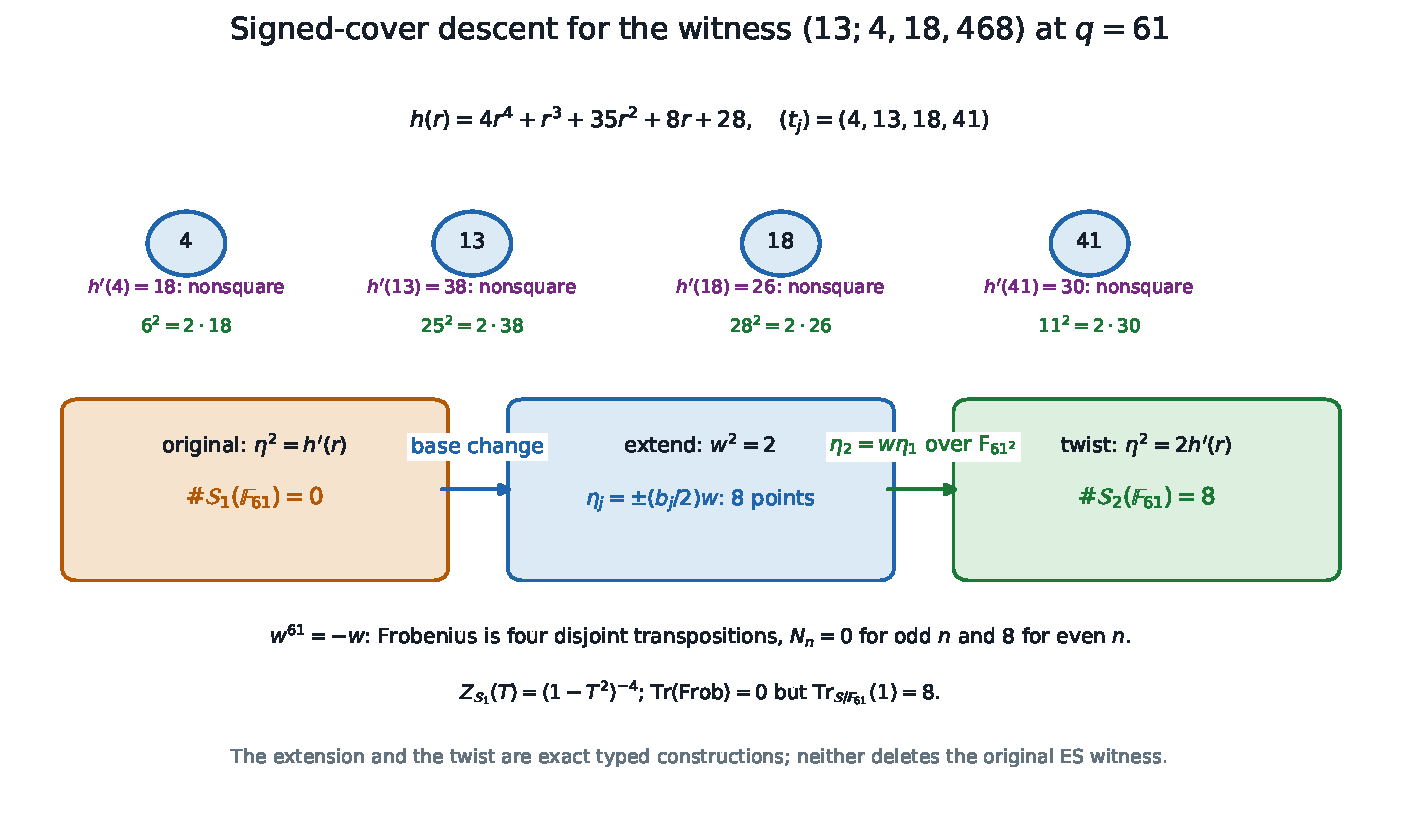
\includegraphics[width=\textwidth]{figures/finite-field-twist-descent.pdf}
\caption{The original signed cover, its quadratic base extension, and the
nonsquare twist for the witness $(13;4,18,468)$ at $q=61$.}
\end{figure}

\clearpage
\input{RESEARCH_CONTINUATION}
\end{document}
